\documentclass{article}
%%%%%%%%%%%%%%%%%%%%%%%%%%%%%%%%%%%%%%%%%%%%%%%%%%%%%%%%%%%%%
% Lecture Specific Information to Fill Out
%%%%%%%%%%%%%%%%%%%%%%%%%%%%%%%%%%%%%%%%%%%%%%%%%%%%%%%%%%%%%
\newcommand{\LectureTitle}{L20: Image Compositing}
%\newcommand{\LectureDate}{\today}
\newcommand{\LectureDate}{March 19, 2015}
\newcommand{\LectureClassName}{CS 557}
\newcommand{\LatexerName}{Peter Henderson}
%%%%%%%%%%%%%%%%%%%%%%%%%%%%%%%%%%%%%%%%%%%%%%%%%%%%%%%%%%%%%

% Change "article" to "report" to get rid of page number on title page
\usepackage{amsmath,amsfonts,amsthm,amssymb}
\usepackage{setspace}
\usepackage{Tabbing}
\usepackage{fancyhdr}
\usepackage{lastpage}
\usepackage{extramarks}
\usepackage{chngpage}
\usepackage{soul,color}
\usepackage{graphicx,float,wrapfig}
\usepackage{afterpage}
\usepackage{abstract}
\usepackage{pgfplots}
\usepackage{caption}
\usepackage{listings}
\usepackage{minted}
\usepackage{url}

% In case you need to adjust margins:
\topmargin=-0.45in
\evensidemargin=0in
\oddsidemargin=0in
\textwidth=6.5in
\textheight=9.0in
\headsep=0.25in
\tikzstyle{cnstyle}=[domain=0:1, samples=100, ultra thick]

% Setup the header and footer
\pagestyle{fancy}
\lhead{\LatexerName}
\chead{\LectureClassName: \LectureTitle}
\rhead{\LectureDate}
\lfoot{\lastxmark}
\cfoot{}
\rfoot{Page\ \thepage\ of\ \pageref{LastPage}}
\renewcommand\headrulewidth{0.4pt}
\renewcommand\footrulewidth{0.4pt}

%%%%%%%%%%%%%%%%%%%%%%%%%%%%%%%%%%%%%%%%%%%%%%%%%%%%%%%%%%%%%
% Some tools
\newcommand{\enterTopicHeader}[1]{\nobreak\extramarks{#1}{#1 continued on next page\ldots}\nobreak
                                    \nobreak\extramarks{#1 (continued)}{#1 continued on next page\ldots}\nobreak}
\newcommand{\exitTopicHeader}[1]{\nobreak\extramarks{#1 (continued)}{#1 continued on next page\ldots}\nobreak
                                   \nobreak\extramarks{#1}{}\nobreak}

\newlength{\labelLength}
\newcommand{\labelAnswer}[2]
  {\settowidth{\labelLength}{#1}
   \addtolength{\labelLength}{0.25in}
   \changetext{}{-\labelLength}{}{}{}
   \noindent\fbox{\begin{minipage}[c]{\columnwidth}#2\end{minipage}}
   \marginpar{\fbox{#1}}

   % We put the blank space above in order to make sure this
   % \marginpar gets correctly placed.
   \changetext{}{+\labelLength}{}{}{}}

\setcounter{secnumdepth}{0}
\newcommand{\TopicName}{}
\newcounter{TopicCounter}
\newenvironment{Topic}[1][Problem \arabic{TopicCounter}]
  {\stepcounter{TopicCounter}
   \renewcommand{\TopicName}{#1}
   \section{\TopicName}
   \enterTopicHeader{\TopicName}}
  {\exitTopicHeader{\TopicName}}

\setcounter{secnumdepth}{0}
\newcommand{\ExampleSectionName}{}
\newcounter{ExampleSectionCounter}[TopicCounter]
\newenvironment{ExampleSection}[1][Example \arabic{ExampleSectionCounter}]
  {\stepcounter{ExampleSectionCounter}
   \renewcommand{\ExampleSectionName}{#1}
   \section{\ExampleSectionName}
   \enterTopicHeader{\ExampleSectionName}}
  {\exitTopicHeader{\ExampleSectionName}}

\setcounter{secnumdepth}{0}
\newcounter{ExampleBoxCounter}[TopicCounter]
\newcommand{\examplebox}[1]
  {
  % We put this space here to make sure we're disconnected from the previous
   % passage
   \stepcounter{ExampleBoxCounter}
   \noindent\fbox{\begin{minipage}[c]{\columnwidth}#1\end{minipage}}\enterTopicHeader{\ExampleSectionName}\exitTopicHeader{\ExampleSectionName}\marginpar{\fbox{\#\arabic{ExampleBoxCounter}}}
   % We put the blank space above in order to make sure this
   % \marginpar gets correctly placed.
   \vskip10pt
   }

\renewcommand{\contentsname}{{\normalsize Topics Covered}}
\renewcommand{\abstractname}{\LectureTitle\ Summary}
\renewcommand{\absnamepos}{flushleft}

\pgfplotsset{vasymptote/.style={
    before end axis/.append code={
        \draw[densely dashed] ({rel axis cs:0,0} -| {axis cs:#1,0})
        -- ({rel axis cs:0,1} -| {axis cs:#1,0});
    }
}}

%%%%%%%%%%%%%%%%%%%%%%%%%%%%%%%%%%%%%%%%%%%%%%%%%%%%%%%%%%%%%

\begin{document}
\begin{spacing}{1.1}
\newpage

% When topics are long, it may be desirable to put a \newpage or a
% \clearpage before each Topic environment
%\newpage
\begin{Topic}[Image Compositing \Roman{TopicCounter}]
Many computer graphics techniques use real images in some way. We have seen several examples: scanned 3D models; texture mapping using photos; environment mapping. Let's start today's lecture with another example.

\subsection{Image Segmentation}
Classic computer (and human) vision problem: Partition an image into regions. It is a difficult problem (and not so well defined). A specific revision to this problem is differentiating foreground from background. A computer graphics application of this problem is that the foreground can then be pasted over a different background (``compositing''). This is an old idea e.g. \textbf{chroma-keying} (green or blue screen).

\subsection{Chroma Keying}
General Approach\\
\begin{itemize}
\item Step 1: Take picture of background B (not necessarily green screen)
\item Step 2:
\item Take image/video of foreground character in front of background (F over B)
\item Step 3: Compute foreground mask
\begin{itemize}
\item For each pixel
\begin{itemize}
\item if (F over B)(x,y) == B(x,y)
\item mask(x,y) = 0 // background
\item else mask(x,y) = 1 // foreground
\end{itemize}
\end{itemize}
\item Write foreground image over a new background Bnew
\begin{itemize}
\item For each pixel (x,y)
\begin{itemize}
\item if mask(x,y) == 1
\item I(x,y) = F(x,y)
\item else I(x,y) = Bnew(x,y)
\end{itemize}
\end{itemize}
\end{itemize}
\subsubsection{Why doesn't it always work?}
\begin{itemize}
\item Cast shadows (foreground object can change background)
\item Interreflections (green screen can reflect, so foreground takes on color of background)
\item Foreground object might happen to have same color as background (in Step 3)
\item Soft edges become hard (mask) e.g Hair and furry object boundaries are difficult to model with a binary mask. That's why you need to take into account the transparency ($\alpha$)
\end{itemize}

\subsection{Alpha}
Think of a pixel as a little square. The occupancy or coverage of a pixel is called $\alpha$.
\begin{itemize}
\item $\alpha = 0$ means not occupied at all (transparent).
\item $\alpha = 1$ means fully occupied (opaque)
\item $0 < \alpha < 1$ means partially occupied
\end{itemize}
In representing RGB images is common to include a 4th component to indicate how much of the pixel is occupied, so we have RGBA. Typically one uses 8 bits for each ``channel'' so this gives 32 bits per pixel.\\\\
\textbf{How do we darken a pixel without changing its opacity ?}
$$\text{darken}(I_{rgba}, \phi) = (\phi I_r, \phi I_g, \phi I_b, I_\alpha)$$
\\
\textbf{How do we change the opacity of a pixel without changing the underlying color (sometimes called ``dissolve")?}
$$\text{dissolve}(I_{rgba}, \delta) = (\delta I_r, \delta I_g, \delta I_b, \delta I_\alpha)$$
\subsubsection{Where do alpha values come from ?}
In OpenGL, we can define surfaces as partially transparent.
\begin{minted}{python}
diffuse_material = [ 1, 0, 0, 0.5 ]
glMaterial(GL_FRONT, GL_DIFFUSE, diffuse_material)
drawPolygon()
\end{minted}
The material has a red color with 50\% transparency.

\subsubsection{F over B}
Let's look at the ``over" operation more formally.
How to put a foreground RGBA layer over a background RGBA layer?
I will use lower case ``rgb" instead of RGB (for reasons to be explained later - namely using ``premultiplied" values).

$$(r, g, b, \alpha) = (\alpha R, \alpha G, \alpha B, \alpha)$$
How to compute a new RGBA layer which is the foreground layer over the background layer.\\
% TODO: might be worth including the slides on transparency and painter's algorithm
\textbf{Special but common case (opaque background):}\\
background is opaque, $B_\alpha = 1$\\
foreground may be partly transparent, $0 < F_\alpha < 1$
$$(F over B)_\alpha = F_\alpha + (1-F_\alpha)B_\alpha = 1$$

\textbf{More general case:}
Background may be partly transparent, $0 \le B_\alpha \le 1$\\
Foreground may be partly transparent, $0 \le F_\alpha \le 1$. Again, given $F_{rgb}$ and $B_{rgb}$, how do we define $(F \text{ over } B)_{rgba}$? (Note this is a per-pixel definition.)

RGB is the color that is computed when rendering e.g. with Blinn-Phong or glColor().\\
The $\alpha$ is given in the definition of the surface material or in glColor() as in our early example with cyan and yellow triangles.\\
\textit{(ASIDE: Note the similarly to homogeneous coordinates. e.g. $(wx, wy, wz, w)$ represents the 3D point (x, y, z).)}

If you're already using pre-multiplied values:

$$(F \text{ over } B)_{rgb} = F_{rgb} + (1-F_\alpha)B_{rgb} = F_\alpha F_{RGB} + (1-F_\alpha) B_\alpha B_{RGB}$$

If you insist on keeping it in not pre-multiplied form then the equation becomes:

$$(F \text{ over } B)_{RGB} = \frac{F_\alpha F_{RGB} + (1-F_\alpha) B_\alpha B_{RGB}}{F_\alpha + (1-F_\alpha)B_\alpha}$$

We are distinguishing two representations: (1) RGBA surface properties that you declare in OpenGL Here, material and opacity are declared independently (which is preferable from the programmer's perspective). In terms of the graphics pipeline, this is a vertex property. (2) Pre-multiplied pixel color values, rgba, that are written in the image buffer. So there's the programmer's perspective (1) and what actually ends up in calculations (2). The transformation between the two happens in the fragment shader.
\\\\
\textit{[ADDED: this is oversimplified. It doesn't deal with textures which can also be defined as RGBA. ]}

\subsection{OpenGL Blending}
Blending must be enabled, else alpha is ignored and incoming fragment is written over the current pixel.

\begin{center}
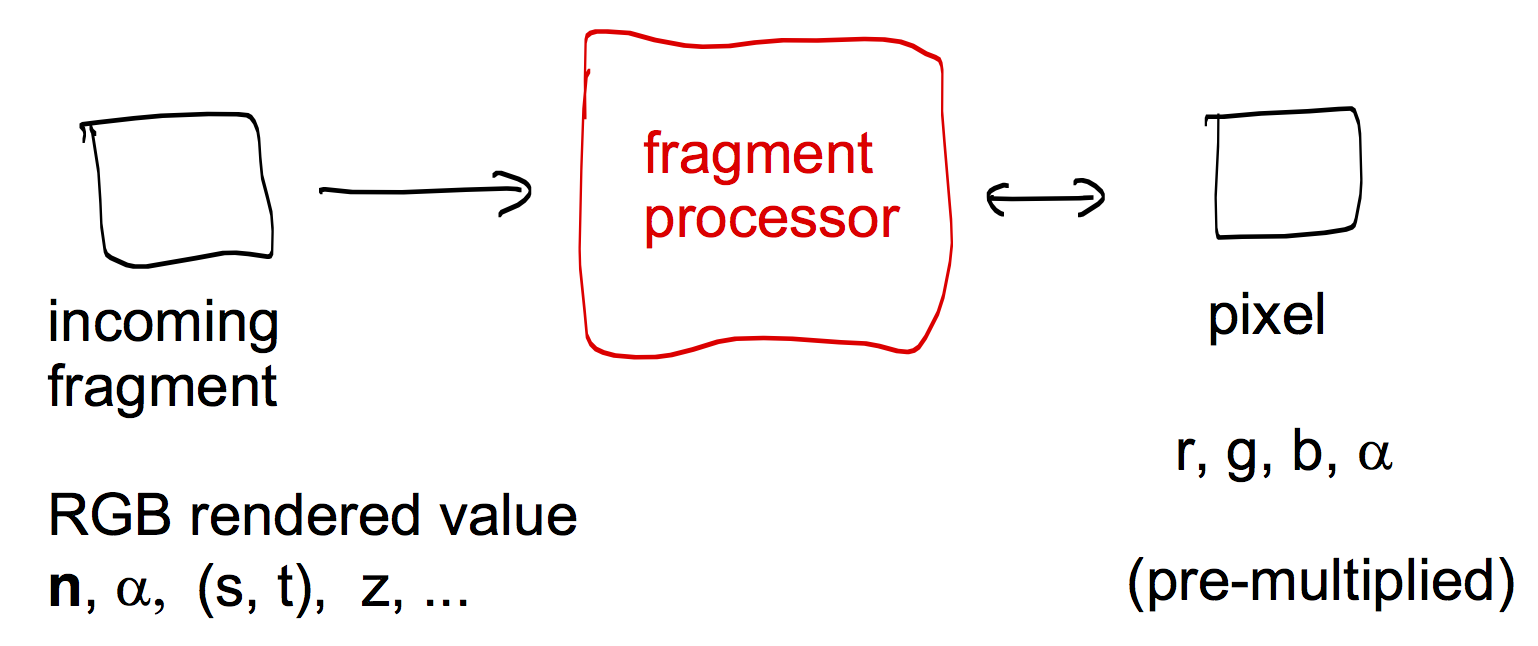
\includegraphics[scale=.3]{images/frag_processor}
\end{center}

The fragment processor takes in fragments and uses them to modify pixels in the frame buffer i.e. image. The fragment processor takes a fragment, and ``blends" it with the current pixel to produce a modified pixel. So in this way you can overlay foreground on background (there's actually a ton of different ways to combine them not just foreground versus background)\footnote{http://www.pegtop.net/delphi/articles/blendmodes/intro.htm}.

\begin{center}
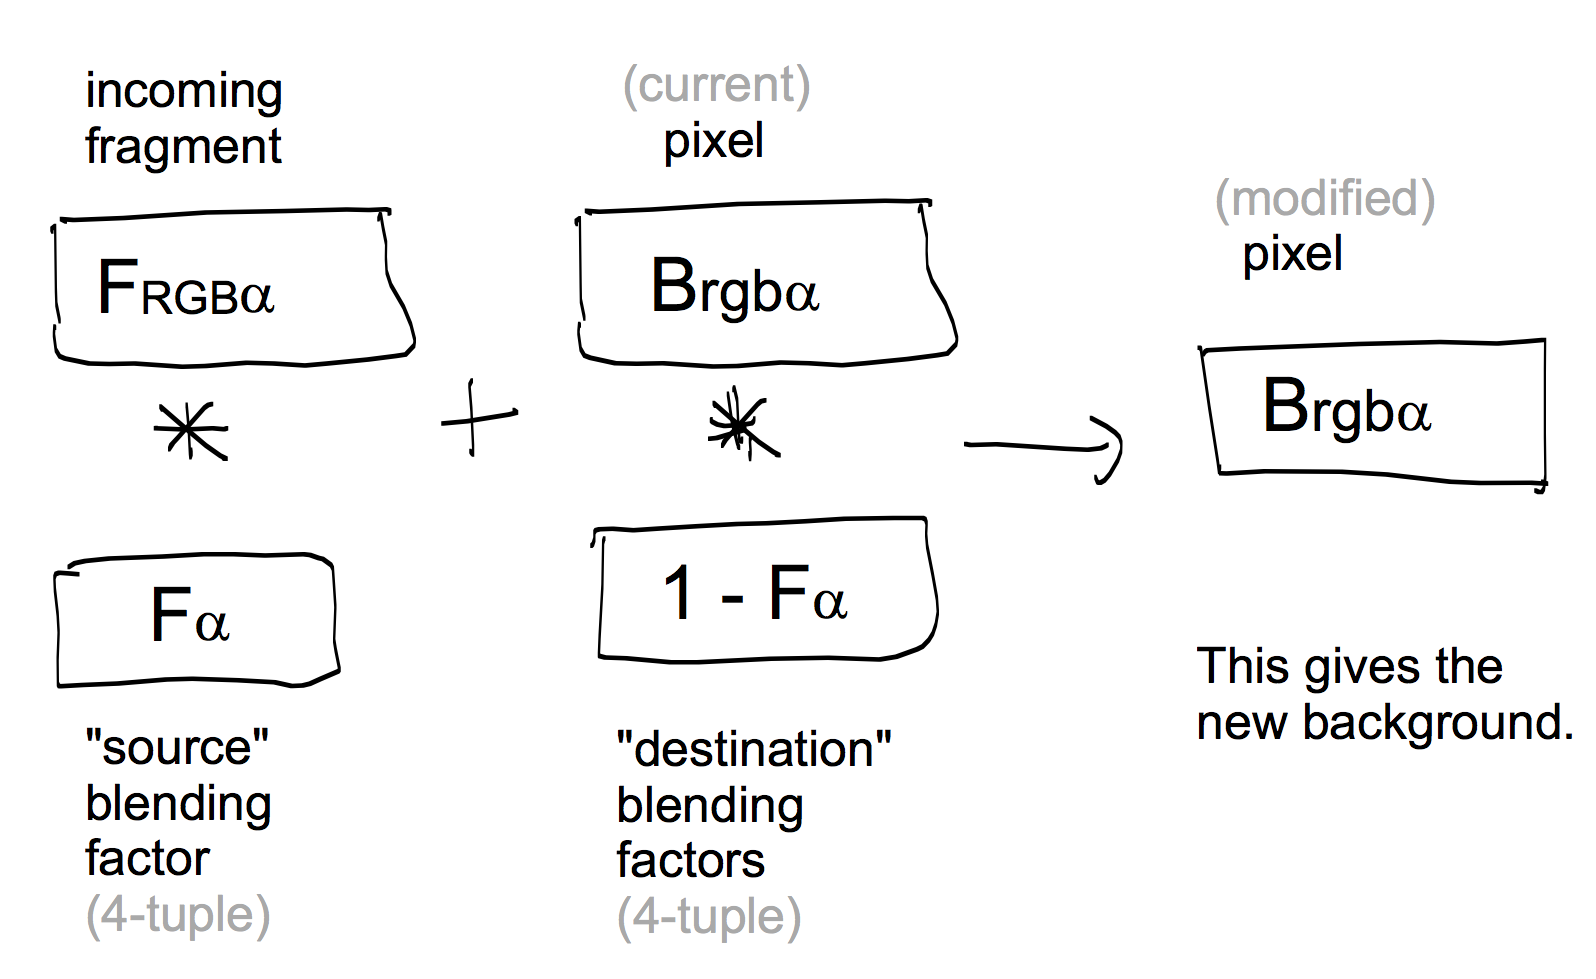
\includegraphics[scale=.3]{images/frag_proc_ex}
\end{center}

Classic OpenGL offers several blending functions.

\begin{minted}{python}
glBlendFunc( source_blending_factor, destination_blending_factor ) For Example 1:
glBlendFunc(GL_SRC_ALPHA, GL_ONE_MINUS_SRC_ALPHA). For Example 2:
glBlendFunc(GL_ONE, GL_ZERO).
\end{minted}

Modern OpenGL allows you to write your own blending functions.

\subsection{Pulling a matte (image processing)}
(alpha channel = a ``matte", binary alpha channel = a ``mask")\\
We are given $(F over B)rgb\alpha$ and maybe something else. We would like to: (1) compute $F_{rgb\alpha}$, (2) given a new new background B', compute $(F over B' )_{rga\alpha}$. However, extracting the foreground is an extremely hard problem.

\subsubsection{Alpha estimation using computer vision}
Use one image only and want to extract RGBA from it.
\\\\
\textbf{Show you have 7 unknown variables at each pixel (but only 3 knowns, namely RGB).}\\\\
Assume: F and B have non-overlapping different distributions of colors in 3D color space.\footnote{Ruzon, Mark A., and Carlo Tomasi. ``Alpha estimation in natural images." 2000}
Allowed: user marks by hand regions that that are B and other regions that are in F (and regions that may be in either).
This partitions the image pixels into three regions, called a ``tri-map".\footnote{Wang, Jue, and Michael F. Cohen. ``Optimized color sampling for robust matting." 2007}

An example of this is the line marking system for American Football\footnote{http://www.sportvision.com/media/1st-and-ten\%E2\%84\%A2-line-system}. This is actually a complex task that involves a lot of the material previously mentioned.
\end{Topic}

\end{spacing}
\end{document}